\documentclass[11pt]{article}
\usepackage[utf8x]{inputenc}
\usepackage{multicol}
\usepackage{float}
\usepackage{cleveref}
\usepackage{nopageno}
\usepackage[margin=1.5cm,a4paper]{geometry}
\newgeometry{left=1.5cm,right=1.5cm,top=1.0cm,bottom=1.5cm}
\usepackage{graphicx}
\newcommand{\HRule}{\rule{\linewidth}{0.5mm}}

\begin{document}
\begin{center}
    \rule{18cm}{0.03cm} \\ [0.35cm]
    \textbf{\Huge{Operation of the First Nuclear Reactor}} \\
    \rule{18cm}{0.04cm} \\
\end{center}

\begin{multicols}{2}

\noindent{By \textbf{L. R. Tomaszewski}} \hspace{1.1cm} 01$^{st}$ December 2019 \\ [-0.2cm]
\rule{9cm}{0.03cm} \\ [-0.45cm]

\noindent{\textbf{With the outbreak of World War Two, scientists in the Manhattan Project dared the near impossible, starting a chain of events that would lead the human race into the atomic age. The goal? To harness and weaponize atomic energy.}} \\ [-0.47cm]

Beginning in 1939, hitherto many nuclear and atomic theories were deemed physically credible, it was only until Otto Hahn and Fritz Strassman discovered nuclear fission was harnessing atomic energy a reality. Fission occurs when atoms nuclei collide each other and lighter nuclei to emerge with two or three neutrons in its nucleus shown in \cref{Chain Reaction}, with each collision a new generation of weaker nuclei is made with few electrons doubling the chances of further collisions, all of these create large amounts of energy that can be harnessed, exploited and controlled\cite{NucPhys}. \\
\indent They discovered the best atoms for nuclear fission were the rare isotope uranium 235 as it was easier to split upon impact and yields greater energy than its brother uranium 238. But with the energy created by fission spreads outwards, a moderator is found to confine and slow the neutrons down. Due to its high temperature resistance, its ability to slow neutrons down as they reflect of its surface and the vast quantity available, graphite is chosen as a suitable moderator \cite{Fermi}. Fermi utilized nuclear fission and envision criticality, where a sustainable nuclear chain reaction takes place in which each fission collision exerts enough neutrons to sustain further series of fission collisions, thus becoming sustainable. \\ [-0.5cm]

\begin{figure}[H]
\centering
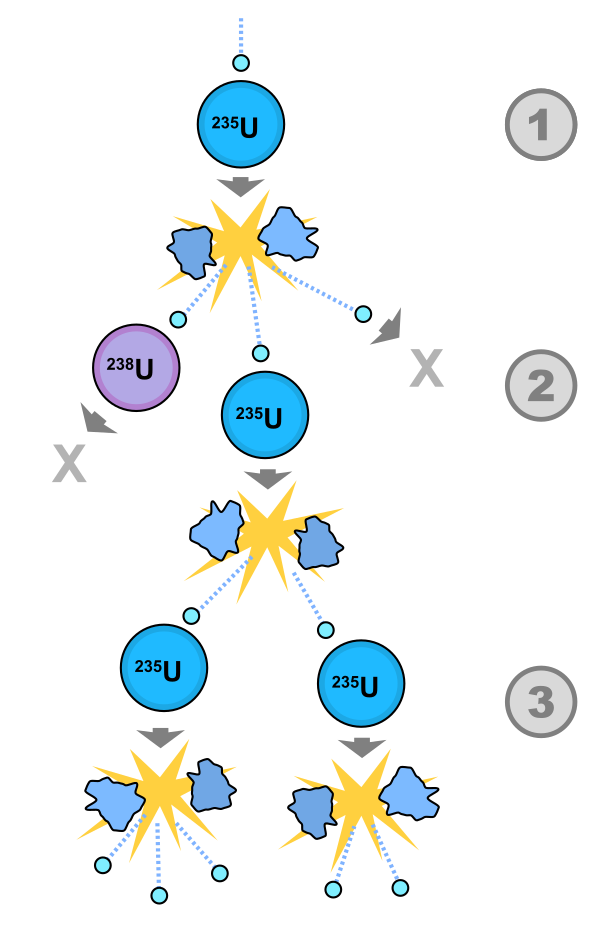
\includegraphics[scale=0.2]{Images/Fission_chain_reaction.png}
\caption{Nuclear Fission Chain Reaction. \cite{ChainReact}}
\label{Chain Reaction}
\end{figure} 
\vspace{-0.5cm}

\begin{center}
    \rule{9cm}{0.05cm} \\ [0.2cm]
    \textbf{\Large{Nuclear Fission discovered!}} \\
    \textbf{Manhattan Project forsees atomic age.} \\ 
    \rule{9cm}{0.1cm}\\ [-0.1cm]
\end{center} 
\vspace{-0.2cm}

\noindent With Europe in turmoil, the United States founded the Manhattan Project, its aim to explore, harness and weaponize atomic energy \cite{TMP}.
Experiments began under the guidance of Enrico Fermi, George Pilgrim, Leo Szilard and Herbert Anderson at the University of Columbia \cite{Fermi} in the United States where due to dwindling resources of uranium and graphite at the time, physical eight foot cubed piles were constructed where in each pile the graphite was more pure and the uranium richer than their forerunners. The graphite was machined to provide a smooth reflective surface and so piles were built, graphite blocks placed in a lattice structure, originally cubed shaped but later they obtained that a spherical shape with machined graphite increased the balance of neutrons and caused very little loss of neutrons per generation which enhances more atomic collisions which are needed to create energy.\\ [-0.8cm]

\begin{center}
    \rule{9cm}{0.05cm} \\ [0.3cm]
    \textbf{\Huge{UNITED STATES DECLARES WAR!}} \\
    \textbf{US rely on Manhattan Project to end the war.} \\ 
    \rule{9cm}{0.1cm}\\ [-0.1cm]
\end{center} 
\vspace{-0.1cm}

\noindent Following the devastating attack on Pearl Harbour, the Manhattan Project gained more interest and funding resulting in an extensive search for purer and richer materials, securing several graphite suppliers and a uranium ore mine in Canada. Relocating to an old, disused squash court underneath the University of Chicago football stadium, 20-30 test piles were constructed, all of different diameters with purer and richer materials. The piles were monitored to observe the energy intensity to determine the best diameter for criticality to occur. After 30 test piles were created the most ideal diameter was found, 15 feet wide and 15 feet high, a monster with a violent uranium heart, able to create a vast amount of energy was one step closer to becoming a reality, the testing was over. \\ 
\indent In October 1942 the 31st and final pile was constructed. In \cref{Chicago Pile 1} blocks of pure, machined smooth graphite filled with uranium slugs buried into the 4 inch squared, foot long bar of carbon surrounding a rich, pure uranium centre standing tall on wooden stilts with a diameter of 25 feet consisting of 400 tons of graphite, 50 tons of uranium and 22,000 slugs of uranium oxide \cite{Youtube}. This was built within a cloth fabric balloon to keep the nitrogen in the atmosphere out to ensure the purity of the fission reactions but this was proved unnecessary \cite{Fermi}. \\ 
\indent Thick rods of cadmium were placed into the heart of the uranium core, cadmium absorbs high rates of neutrons that can stop fission chain reaction taking place. Two cadmium rods were controlled mechanically to act as the switch, turning the reactor on or off, a thin third rod is pulled or pushed in and out by a human operator, this rod is thin enough to increase or decrease the number of fission reactions but not thick enough to stop the reaction from taking place, just enough to control the nuclear fission taking place. A fourth cadmium rod, the thickest of all attached to a rope and weight and is placed so that it strikes deep into the uranium heart so that in an emergency the nuclear fission can be stopped dead, if this fails then a cadmium salt solution is ready to flood the uranium chamber and cease the fission reactions. \\

\begin{figure}[H]
\centering
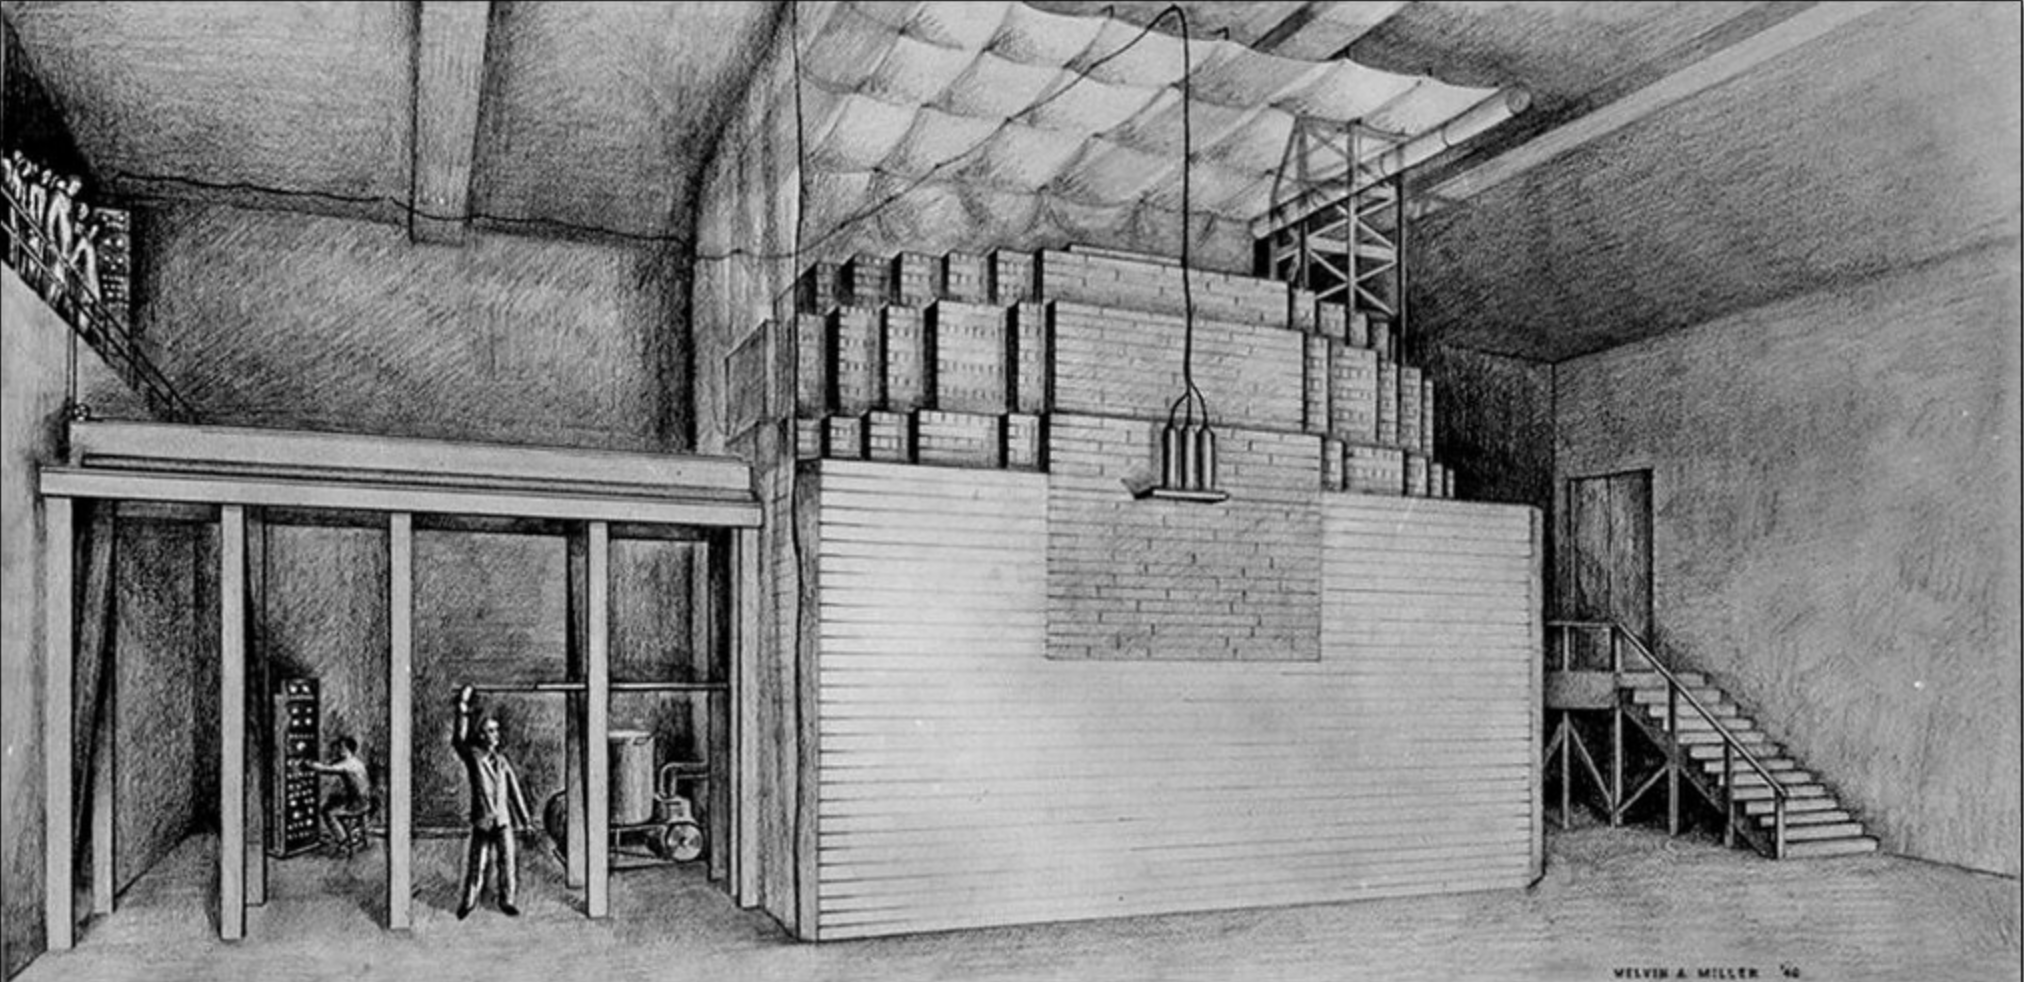
\includegraphics[scale=0.24]{Images/CP-1.png}
\caption{Construction of Chicago Pile 1. \cite{Picture}}
\label{Chicago Pile 1}
\end{figure} 

\noindent On the 2$^{nd}$ December 1942 with construction finished on the pile designated 'Chicago Pile 1' (CP-1). Its uranium core has already created small fission reactions which the cadmium rods stopped but Fermi wanted to ensure that CP-1 did not reach criticality before they had finished construction. But with CP-1 ready, the cadmium rods were carefully removed and as each one was removed the number of fission reactions increased and the intensity of the energy exerted off the fission reaction grew, when all the cadmium rods were removed the intensity rose rapidly creating concern but after a few minutes it stabilized at a finite level. Only when all the cadmium rods were inserted back into the uranium filled graphite ball did Fermi and the other scientists realise how easy the prototype was to control, the intensity could be adjusted with extreme accuracy to any desired level. Even though graphite can withstand high thermal temperatures, there was no shield for the heat that was created from the fission process so it was predicted that CP-1 could operate at a nominal power, never exceeding 200 watts of power but Fermi had succeeded in creating a nuclear power source and found it easy to control. \\ [-1.0cm]

\begin{center}
    \rule{9cm}{0.05cm} \\ [0.2cm]
    \textbf{\Large{First nuclear reactor works, stable chain reaction obtained!}} \\
    \textbf{Human race welcomes atomic age.} \\
    \rule{9cm}{0.1cm}\\ [-0.1cm]
\end{center} 
\vspace{-0.2cm}

\noindent In the aftermath of CP-1, many nuclear reactors emerged, some researching power, many researching weaponizing the atomic energy, it was only with the help of CP-1 that plutonium was made in large quantities. Plutonium being the radioactive heart of the three atomic bombs the united states planned to drop on Japan in 1945, where two of them were used and successfully ended the war and showed the horror or weaponizing atomic energy. After World War Two came to an end the Manhattan Project shut down and Fermi still served on the 'General Advisory Committee' and strongly opposed the use of weaponizing nuclear energy. But 77 years on where atomic energy powers a majority of the worlds countries, supplying the human race with a reliable source of energy and huge advancements in the medical field, Fermi and his group of scientists set out to weaponize atomic energy but instead opened a door to the atomic age, a defining scientific event in the 20th century.  

\end{multicols}
\newpage
\bibliographystyle{plain}
\bibliography{mybib.bib}
\end{document}